\documentclass[12pt]{article}
\usepackage{geometry}
 \geometry{
 a4paper,
 total={170mm,257mm},
 left=20mm,
 top=20mm,
 }
\usepackage{amsmath}
\usepackage{amssymb}
\usepackage{graphicx}
\usepackage{hyperref}
\usepackage{cleveref}
\usepackage[most]{tcolorbox}
\usepackage[utf8]{inputenc}
\usepackage{tikz}
\usepackage{pstricks-add}
\usepackage{enumerate}
\usepackage{MnSymbol}
\usepackage{mathtools}
\usepackage{subcaption}
\DeclarePairedDelimiter\ceil{\lceil}{\rceil}
\DeclarePairedDelimiter\floor{\lfloor}{\rfloor}
\DeclarePairedDelimiter\abs{\left|}{\right|}
\hypersetup{
    colorlinks=false,
    pdfborder={0 0 0},
}
\newcommand\tab[1][1cm]{\hspace*{#1}}
\newtheorem{theorem}{Theorem}
\usetikzlibrary{arrows,calc}
\title{MAT 1001: Calculus I}
\author{Alfonsus Rodriques Rendy}
\date{2021-9-9}

\begin{document}
\begin{center}
    \hspace*{-0.5cm}
    \framebox{
    \begin{minipage}{1\linewidth}
        \textbf{MAT1001 Calculus I} \\
        \vspace{-0.8cm}
        \begin{center}
            \huge{Lecture 2 - 3: Limits} 
            \\
            \vspace{0.5cm}
            \normalsize \textit{Lecture by Dr. Arjan Abeynaike} \\
            \vspace{0.3cm}
            \text{Scribe by Alfonsus Rodriques Rendy} \\
            \textrm{Sep 9, 2021 - Sep 16, 2021}
        \end{center}
    \end{minipage}}
\end{center}

\section{Limits}
\subsection{Definition}
\paragraph{Definition} Let $f : D \rightarrow \mathbb{R}$ be a function "near" $x=c$, we write
\[
    \lim_{x \to c} f(x) = L
\]
if $f(x)$ can get arbitrarily close to $L$ for all $x$ close enough to $c$.
\paragraph{Limits Existence} $\lim_{x \to c} f(x)$ exists if and only if:
\begin{enumerate} 
    \item $\lim_{x \to c^+} f(x)$ exists
    \item $\lim_{x \to c^-} f(x)$ exists
    \item $\lim_{x \to c^-} f(x) = \lim_{x \to c^+} f(x) = L$, such that $L \in \mathbb{R}$ 
\end{enumerate}
In other words, as $x$ approaches $c$ from the left, the value of $f(x)$ is approaching the same value of $L \in \mathbb{R}$
that $f(x)$ is approaching when $x$ approaches $c$ from the right. Note that that $\pm \infty$ do not count as a limit here (because they are not
real numbers).
\paragraph{Delta-Epsilon Definition} Let $f : D \rightarrow \mathbb{R}$ be a function defined on an open iterval 
containing c, except possibly  at c itself.
Let $L \in \mathbb{R}$ so $L \neq \pm \infty$, then we write:
\[
    \lim_{x \to c} f(x) = L
\]

\[
    \textrm{If, for all } \epsilon > 0 \textrm{, there exists } \delta > 0 \\
\]
\[
    \textrm{ such that for all } x \in D \textrm{ , we have } 0 < |x-c| < \delta \Rightarrow |f(x) - L| < \epsilon
\]

\begin{figure} 
    \centering
    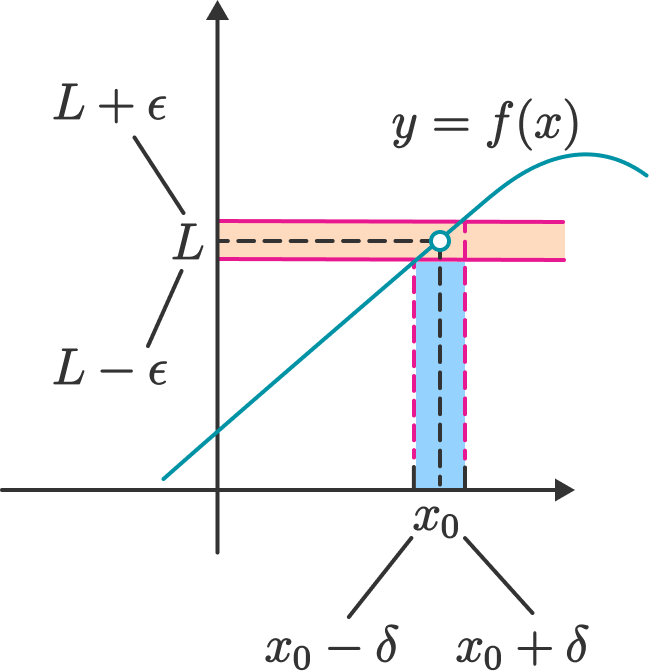
\includegraphics[width=0.4\linewidth]{images/limit_def.png}
    \caption{Illustration of the precise definition of limit}
\end{figure}

\paragraph{Example} Use the formal definition of limits to show that 
\[
    \lim_{x \to 2} x^2 = 4
\]
Let $\epsilon > 0$. We want find $\delta > 0$ such that $|x^2 - 4| < \epsilon$ 
given that $0 < |x-2| < \delta$ for all $x \in D$.

\noindent
Consider 
\begin{align*} 
    |x^2 - 4| < \epsilon \rightarrow |x - 2|\cdot|x + 2| < \epsilon \rightarrow |x - 2| < \frac{\epsilon}{|x + 2|} 
\end{align*}

\noindent
Note that $\epsilon$ is a very small number, so $\delta$ is also very small. We can assume that 
$\delta < 1$, then $|x - 2| < 1 \rightarrow 1 < x < 3$\\
We have
\begin{align*} 
    & \frac{1}{5} < \frac{1}{|x - 2|} < \frac{1}{3} \\
    & \frac{1}{5} < \frac{1}{|x - 2|} \\
    & \frac{\epsilon}{5} < \frac{\epsilon}{|x - 2|} 
\end{align*} 

\noindent
If we assume that $\delta \leq \frac{\epsilon}{5}$ and $|x - 2| < \delta$:
\begin{align*} 
     |x - 2| &< \delta \\
     |x - 2| &< \frac{\epsilon}{5} \\
     |x - 2|\cdot|x + 2| &< |x + 2|\cdot \frac{\epsilon}{5} <  |x + 2|\cdot \frac{\epsilon}{|x + 2|} = \epsilon
\end{align*}
Hence, given $\epsilon > 0$, set $\delta \leq \epsilon / 5$. Then  $|x - 2| < \delta$  implies that $|x^2 - 4| < \epsilon$ 
for all $x \in D$. This shows that $\lim_{x \to 2} \; x^2 = 4$ \\ \\

\begin{figure}[h!]
    \centering
    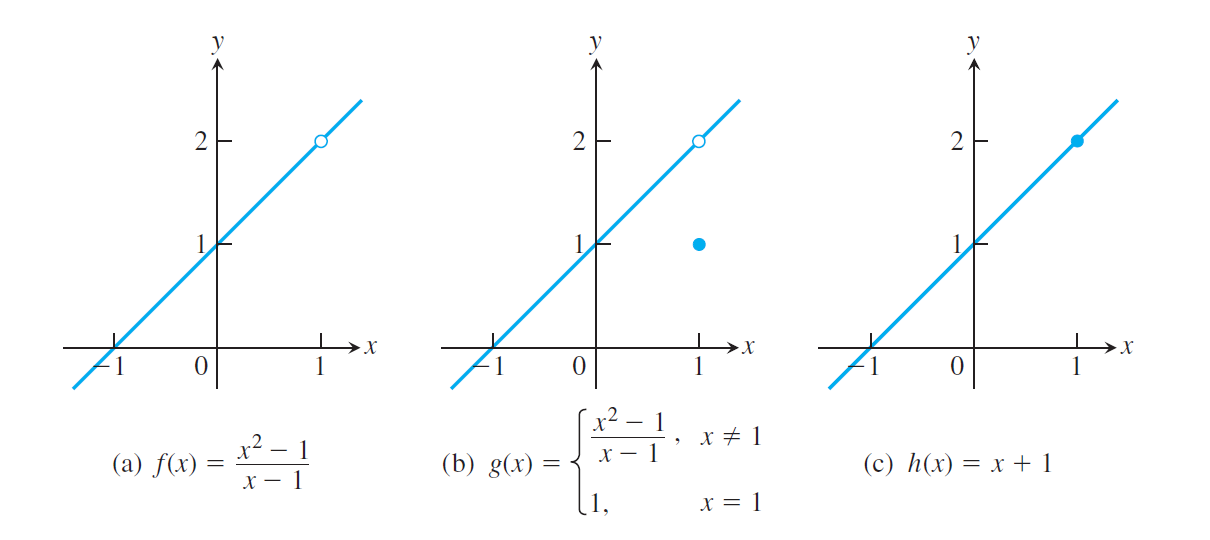
\includegraphics[width=0.8\linewidth]{images/limit and function.png}
    \caption{Limit of $f(x)$, $g(x)$, and $h(x)$ all equal to 2 as x approaches 1, but only $h(x)$ have $h(1) = 2$ }
\end{figure}

\noindent
Note that the limit of $f(x)$ as $x$ approaching $c$ has no relation with the value
of $f$ at $c$. In fact, even if $f(c)$ is undefined, $f$ may still have a limit
at $c$. We can write
\[
    \lim_{x \to c} f(x) \neq f(c)
\]

\subsection{Properties of limit}
\begin{theorem}[Properties of Limits]
    \label{properties}
Let $L$, $M$, $c$, $k$ $\in \mathbb{R} $, and $f$ and $g$ be functions such that
\[
    \lim_{x \to c} f(x) = L \textrm{ and } \lim_{x \to c} g(x) = M
\]
Then:
\begin{itemize} 
     \item $\lim_{x \to c} \: (f(x) \pm g(x)) = L + M$
     \item $\lim_{x \to c} \: (f(x) \cdot g(x)) = L \cdot M$
     \item $\lim_{x \to c} \: \frac{f(x)}{g(x)} = \frac{L}{M}$, provided that $M \neq 0$.
     \item $\lim_{x \to c} \: k.f(x) = k.L$
     \item $\lim_{x \to c} \: [f(x)]^n = L^n$, $n$ is a positive integer
     \item $\lim_{x \to c} \: \sqrt[n]{f(x)} = \sqrt[n]{L} = L^{1/n}$, $n$ is a positive integer, \\ If $n$ is even then we
     assume that $f$ is positive in some open interval containing $c$.
\end{itemize}
\end{theorem}

\begin{theorem}[Limits of Polynomials] 
    If $P(x)$ is a polynomial function, that is if there exists real numbers $a_1$, ..., $a_n$ 
    such that 
    \[
        P(x) = a_{n}x^{n} + a_{n - 1}x^{n - 1} + ... + a_{0}
    \]
    then
    \[
        \lim_{x \to c} P(x) = p(c) \textrm{ for any polynomial function p}.
    \]
\end{theorem}
\begin{theorem}[Limits of Rational Functions]
    \label{rational}
    If $p$ and q are polynomial functions on $\mathbb{R}$, then for any $c \in \mathbb{R}$
    such that $q(c) \neq 0$, then
    \[
        \lim_{x \to c} \frac{p(x)}{q(x)} = \frac{p(c)}{q(c)}\, 
    \]
\end{theorem}
\subsection{One-sided Limits}
If $f$ is defined on some interval $(c, c + a)$, then we have a \textbf{right-hand limit}:
\[
    \lim_{x \to c^+} f(x) 
\]
We say "limit of $f(x)$ as $x$ approaches $c$ from the right". \\
If $f$ is defined on some interval $(c - a, c)$, then we have a \textbf{left-hand limit}:
\[
    \lim_{x \to c^-} f(x) 
\]
We say "limit of $f(x)$ as $x$ approaches $c$ from the left".

\begin{theorem}[Equalled One-Sided Limits]
    Let $c \in R$ and $L \in R$, and let $f$ be a function defined on some
    open interval $D$ containing $c$, except possibly at $c$. Then
    \[
        \lim_{x \to c} f(x) = L \Leftrightarrow \lim_{x \to c^ -} f(x) = \lim_{x \to c^+} f(x) = L
    \]
\end{theorem}
\section{Continuity}
\subsection{Definition}
\paragraph{Definition} Let $f : D \rightarrow \mathbb{R}$ be a function defined on
an open interval containing c, we say $f$ is continuous at $c$ if 
\[
    \lim_{x \to c} f(x) = f(c)
\]

\noindent
Precise definition: Let $f : D \rightarrow \mathbb{R}$ be a function, where $D$ is an interval, and let
$c \in D$. Then $f$ is said to be continuous at $c$ if for every $\epsilon > 0$,
there exists a $\delta > 0$ such that 
\[
    |f(x) - f(c)| < \epsilon \textrm{ for all } x \in D \textrm{ satisfying } |x - c| < \delta
\]
\noindent
If $f$ is not continuous at $c \in D$, then we say that $f$ is
discontinuous at $c$. We say that $f$ is continuous on $D$ if it is
continuous at every point in $D$. \\ \\
\noindent
Functions that are continuous at every $c \in \mathbb{R}$ are:
\begin{itemize} 
     \item Constant function: $f(x) = k$ , where $k$ is constant, $D \in \mathbb{R}$.
     \item Identity function: $f(x) = x$, $D \in \mathbb{R}$.
     \item Absolute value function: $f(x) = |x|$, $D \in \mathbb{R}$.
     \item Natural exponential function: $f(x) = e^x$, $D \in \mathbb{R}$.
     \item Natural logarithmic function: $f(x) = \ln x$, $D = \{x \in \mathbb{R} : x > 0\}$.
     \item Basic trigonometric functions: $f(x) = \sin x$, $g(x) = \cos{x}$, $D \in \mathbb{R}$.
\end{itemize}
\subsection{One-sided Continuity}
\paragraph{Definition} Let $f : D \rightarrow \mathbb{R}$ be a function, where $D$ is an interval, and let
$c \in D$. We say that $f$ is \textbf{right-continuous} at $c$ if $\lim_{x \to c^+} \; f(x) = f(c)$.
We say that $f$ is \textbf{left-continuous} at $c$ if $\lim_{x \to c^-} f(x) = f(c)$. \\

\noindent
From the definition of one-sided continuity, we can define that 
a function $f : [a,b] \rightarrow \mathbb{R}$ is continuous if $f$ is continuous at
every $c \in (a,b)$, left-continuous at $b$, and right-continuous at $a$.

\begin{figure}[h!]
    \centering
    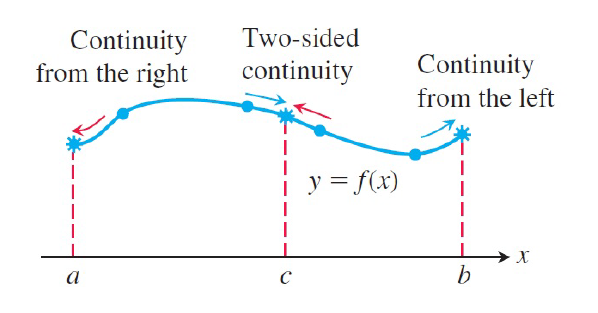
\includegraphics[width=0.5\linewidth]{images/continuity.png}
    \caption{Continuity at point $a$, $b$, and $c$}
\end{figure} 

\subsection{Properties}
\begin{theorem}[Combinations of Continuous Functions]
    Let $f$ and $g$ be functions. If both $f$ and $g$ are continuous at a
    point $c$, then so are the functions $f + g$, $f - g$, $f \cdot g$ and $f / g$. (For
    $f / g$, we assume that $g(c) \neq 0$.)
\end{theorem}
\begin{theorem}[Limit of Continuous Functions]
    Let $f$ and $g$ be functions, such that $g \circ f$ is defined. Suppose that
    $g$ is continuous at a point $b$ and $\lim_{x \to c} f(x) = b$. Then
    \[
        \lim_{x \to c} g(f(x)) = g(\lim_{x \to c} f(x)) = g(b)
    \]
\end{theorem}
\paragraph{Example} 
\begin{align*} 
    g(x) &= \sin x \\
    f(x) &=
    \begin{cases}
        1 & x = 0 \\
        0 & x \neq 0 \\
    \end{cases}
\end{align*}

Since $g$ is continuous at every $c \in \mathbb{R}$ and we have $\lim_{x \to 0} \; f(x) = 0$, then
\[
    \lim_{x \to 1 } g \circ f = g(\lim_{x \to 1} f(x)) = g(0) = \sin 0 = 0
\]
\begin{theorem}[Compositions of Continuous Functions]
    \label{composition continuous}
    Let $f$ and $g$ be functions, such that $g \circ f$ is defined. Suppose that
    $f$ is continuous at $c$, and $g$ is continuous at $f(c)$. Then $g \circ f$ is
    continuous at $c$.
\end{theorem}

\paragraph{Proof of Theorem \ref{composition continuous}} To proof theorem \ref{composition continuous}, we can use the formal definition of limits, that is
for any given $\epsilon = 0$, there exists $\delta > 0$ such that for all $x$ with $|x - c| < \delta$ we have
\[
    |g(f(x)) - g(f(c)) | < \epsilon
\]
By definition of limits
\[
    \lim_{x \to c} \; g(f(x)) = g(f(c))
\] 
Therefore we have
\[
    \lim_{x \to c} \; g \circ f = g \circ f
\]
Hence, by the definition of continuity, $g \circ f$ is continuous at $c$.
\subsection{Discontinuity}
\begin{figure}[h!]
    \centering
    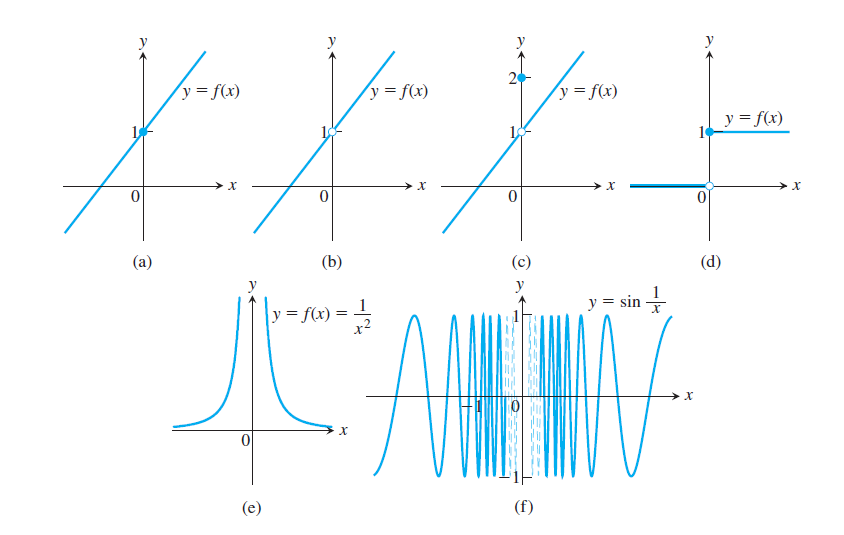
\includegraphics[width=0.7\linewidth]{Images/Discontinuity.png}
    \caption{(a) is continous at 0, (b) and (c) have a removable discontinuity, (d) has a jump discontinuity, 
    (e) and (f) has an essential discontinuity}
\end{figure}

Let $f : D \rightarrow \mathbb{R}$ be a function, where $D$ is an interval containing $c$.
Suppose that $f$ is not continuous at $c$. If $c$ is an interior point of $D$, 
then one of the following is true:
\begin{enumerate}[i] 
     \item The function $f$ has a \textbf{removable discontinuity} at $c$, which
     means that $\lim_{x \to c} \; f(x) = L$ for some $L \in R$, but $L \neq f(c)$. It
     can be made continuous at $c$ by redefining $f(c)$ to be $L$.
     \item The function $f$ has a \textbf{jump discontinuity} at $c$, which
     means that both $\lim_{x \to c^-} f(x)$ and $\lim_{x \to c^-} f(x)$ exists, but not equal.
     \item The function $f$ has a \textbf{essential discontinuity} at $c$, which
     means that at least one of both $\lim_{x \to c^-} f(x)$ and $\lim_{x \to c^-} f(x)$ doesn't exist.
\end{enumerate}
If $c$ is the left endpoint of $D$, then one of the following is true:
\begin{enumerate}[i] 
    \item The function $f$ has a \textbf{jump discontinuity} at $c$, which
    means that $\lim_{x \to c^+} f(x) = L$ but $L \neq f(c)$. It
    can be made continuous at $c$ by redefining $f(c)$ to be $L$.
    \item The function $f$ has a \textbf{essential discontinuity} at $c$, which
    means that $\lim_{x \to c^+} f(x)$ doesn't exist.
\end{enumerate}
The discontinuity is defined similarly if $c$ is the left endpoint of $D$.

\section{Sandwich Theorem/Squeeze Theorem}
\begin{theorem}[The Sandwich Theorem] 
    Suppose that g(x) $f(x) \leq g(x) \leq h(x)$ for all $x$ in some open interval containing
    $c$, except possibly at $x = c$ itself, and suppose we have that
    \[
        \lim_{x \to c} f(x) = \lim_{x \to c} h(x) = L
    \]
    then
    \[
        \lim_{x \to c} g(x) = L
    \]
\end{theorem}

\paragraph{Example} 
\[
    \lim_{x \to 0} x^2 \sin{\frac{1}{x}}
\]
Note that $-1 \leq \sin x \leq 1$ for all $x$ with $x \neq 0$. So,
\[
    - x^2 \leq x^2 \sin {\frac{1}{x}} \leq x^2 \textrm{ for } x \neq 0
\]
Since
\[
    \lim_{x \to 0} - x^2 = \lim_{x \to 0} x^2 = 0
\]
by sandwich theorem we have
\[
    \lim_{x \to 0} x^2 \sin{\frac{1}{x}} = 0
\]

\begin{theorem}
    If $f(x) \leq g(x)$for all $x$ in some open interval containing $c$, except
    possibly at $x = c$ itself, and the limits of $f$ and $g$ both exist as $x$ approaches $c$,
    then
    \[
        \lim_{x \to c} f(x) \leq \lim_{x \to c} g(x) 
    \]
\end{theorem}

\section{Intermediate Value Theorem (IVT)}
\begin{theorem}[Intermediate Value Theorem]
    If $f$ is a continuous function on a closed interval $[a,b]$ and if $y_0$ is any value
    between $f(a)$ and $f(b)$ then $y_0 = f(c)$ for some $c$ in $[a,b]$
\end{theorem}

\begin{figure}[h!] 
    \centering
    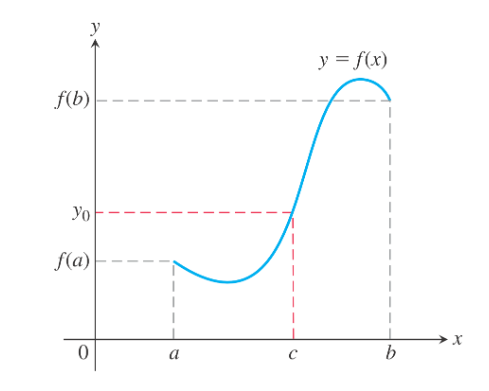
\includegraphics[width = 0.5\linewidth]{Images/ivt.png}
    \caption{Intermediate Value Theorem}
\end{figure}

\paragraph{Example} Show that $x^3 - x = 7$ has a solution \\ \\
To find whether $x^3 - x = 7$ has a solution, it is suffice to show that $x^3 - x - 7 = 0$ \\ \\
Let $f(x) = x^3 - x - 7 $, which is a polynomial function and is continuous for all $x \in \mathbb{R}$. \\ \\
Take two arbitrary point, that is $a = 0$  and $b = 3$. Since $f(0) = -7$ and $f(3) = 17$, $ -7 < 0 < 17 $,
by IVT $\exists \; x_0 \in (0, 3)$ such that $f(x_0) = 0$. \\ \\
Hence, $x_0^3 - x_0 = 7$ has a solution.

\section{Special Limits (Trigonometry)}
There are several special limits in trigonometric function. To solve limits problem
for trigonometric function, we usually use there special limits (try to change the form of the function 
using these special limits). 
\[
    \lim_{x \to 0} \frac{\sin x }{x} = 1
\]
\noindent
To prove this form of limit, we use geometric approach. First we draw a unit circle and try to use
sandwich theorem to proof the limit.
\begin{figure}[h!]
    \centering
    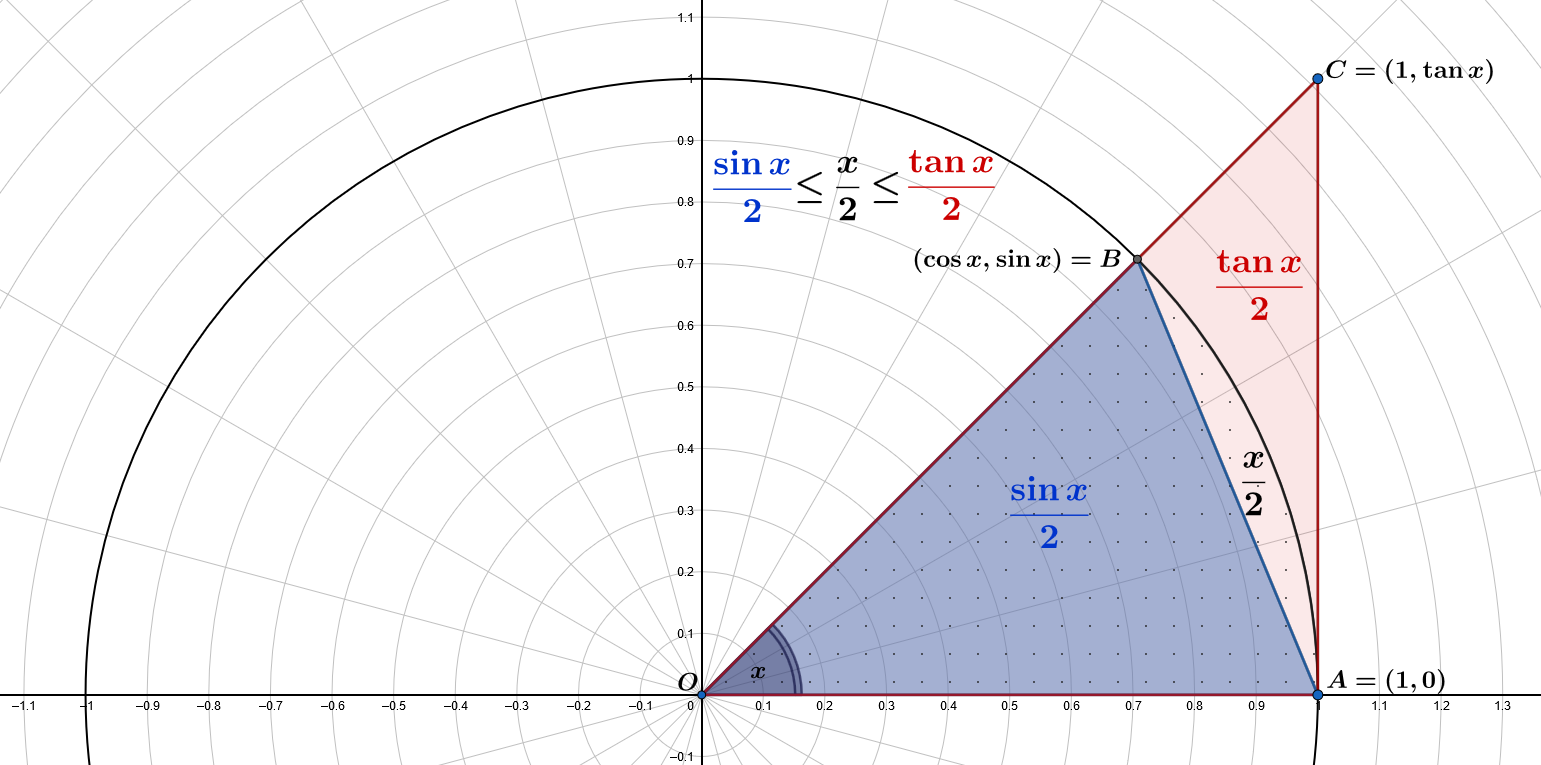
\includegraphics[width = 0.7\linewidth]{Images/proof special limit 1.png}
\end{figure}

\begin{align*} 
    \textrm{Area of }\triangle OAB &= \frac{1}{2} \cdot b \cdot h =  \frac{1}{2} \cdot 1 \cdot \sin x \\
    \textrm{Area of }\downslice OAB &= \frac{x}{2\pi} \cdot \pi \cdot r^2 = \frac{x}{2} \\
    \textrm{Area of }\triangle OAC &= \frac{1}{2} \cdot b \cdot h =  \frac{1}{2} \cdot 1 \cdot \tan x \\
\end{align*}

From the figure we can see that $\triangle OAB \leq \downslice OAB \leq \triangle OAC$ Therefore,
\begin{align*} 
    \frac{\sin x}{2} \leq \frac{x}{2} \leq \frac{\tan x}{2} \\
    \sin x \leq x \leq \tan x \\
    1 \leq \frac{x}{\sin x} \leq \frac{1}{\cos x} \\
    1 \geq \frac{\sin x}{x} \geq \cos x \\
\end{align*}

\noindent
Since
\begin{align*} 
     \lim_{x \to 0} 1 = 1 \textrm{\tab and \tab} \lim_{x \to 0} \cos x = 1
\end{align*}
By sandwich theorem, $\lim_{x \to 0} \frac{\sin x}{x} = 1$
\begin{figure}[h!]
    \centering
    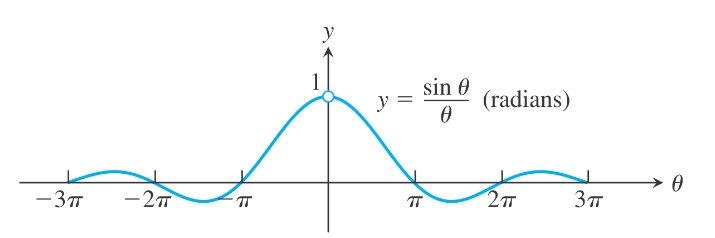
\includegraphics[width = 0.7\linewidth]{Images/limit trigonometry 1.png}
    \caption{Graph of $\frac{\sin x}{x}$}
\end{figure}

\section{Limits Involving Bounded Functions}
\paragraph{Definition} A function $f$ is said to be bounded on S if $\exists \; M \in \mathbb{R}$ such that
$f \leq M \; \forall x \in S$. \\ \\
Example of bounded function is $\sin x$ and $\cos x$ in its domain $D \in \mathbb{R}$ because for all $x \in D$, $f(x) \in [-1, 1]$.

\begin{theorem}[Limits Involving Bounded Function]
    \label{bounded limit}
    Suppose that $f$ and $g$ are functions defined on some open interval $D$ containing $c$ (except possibly at $c$). 
    If $lim_{x \to c} f(x) = 0$ and $g(x)$ is bounded on $D \setminus \{c\}$, then
    \[
        \lim_{x \to c} f(x)g(x) = 0
    \]
\end{theorem}
\paragraph{Proof on Theorem \ref{bounded limit}} $g$ is bounded on $D \setminus \{c\}$, So
\begin{align*} 
    &\Rightarrow \exists \; M \in \mathbb{R} : \; \mid g(x) \mid \leq M, \textrm{\tab} &\forall x \in D \setminus \{c\} \\
    &\Rightarrow 0 \leq \; \mid f(x)\mid \mid g(x)\mid \; \leq M \mid f(x)\mid, &\forall x \in D \setminus \{c\} \\
\end{align*}
\noindent
Since
\[
    \lim_{x \to c} M|f(x)| = M \lim_{x \to c} |f(x)| = 0
\]

\noindent
by sandwich theorem
\[
    \lim_{x \to c} |f(x)||g(x)|= 0
\]

\noindent
Since
\[
    - |f(x)||g(x)| \leq f(x)g(x) \leq |f(x)||g(x)|, \forall x \in D \setminus \{c\} \\
\]

\noindent
by sandwich theorem
\[
    \lim_{x \to c} f(x)g(x)= 0
\]

\paragraph{Example} $\mid \cos x \mid \; \leq 1 \; \forall x \in \mathbb{R}$. Find $\lim_{x \to 5} (x^3 - 25x) \cos{(\log|x-5|)}$ \\ \\
Since $\cos{(\log|x-5|)}$ is bounded for all $x \in \mathbb{R} \setminus \{5\}$ \\
and  $\lim_{x \to 5} (x^3 - 25x) = 0$, then by theorem \ref{bounded limit}
\[
    \lim_{x \to 5} (x^3 - 25x) \cos{(\log|x-5|)} = 0
\]

\section{Limits Involving Infinity}
Infinity $(\infty)$ does not represent a real number. However, we use $\infty$ to describe the behavior 
of a function when the value in its domain / range outgrows all finite bound that is can't be represented by 
a single real value.
\subsection{Finite Limits as $x \to \pm \infty$}
\paragraph{Definition} First, we say that $f(x)$ has the limit $L$ as $x$ approaches infinity and write
\[
    \lim_{x \to \infty} f(x) = L
\]
if, for every number $\epsilon > 0$, there exists a corresponding number $M$ such that for all $x$
\[ 
    x > M \textrm{\tab} \Rightarrow \textrm{\tab} |f(x) - L| < \epsilon
\]
Second, we say that $f(x)$ has the limit $L$ as $x$ approaches minus infinity and write
\[
    \lim_{x \to -\infty} f(x) = L
\]
if, for every number $\epsilon > 0$, there exists a corresponding number $N$ such that for all $x$
\[ 
    x < N \textrm{\tab} \Rightarrow \textrm{\tab} |f(x) - L| < \epsilon
\]

\begin{figure}[h!]
    \centering
    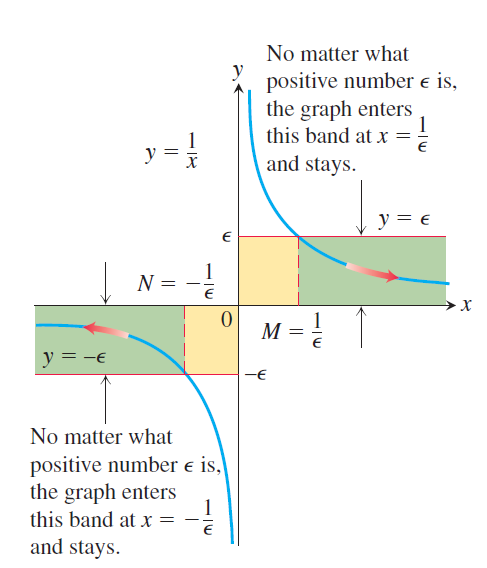
\includegraphics[width = 0.4\linewidth]{Images/infty limit 4.png}
    \caption{Geometry illustration of the limit on infinity definition}
\end{figure}
\paragraph{Example 1} Show that $\lim_{x \to \infty} \frac{1}{x} = 0$
Let $\epsilon > 0 $ be given and let $M = \frac{1}{\epsilon}$. \\ \\
If $x > M = \frac{1}{\epsilon}$, then
\[
    \left|  \frac{1}{x} - 0 \right|  = \frac{1}{x} < \frac{1}{\frac{1}{\epsilon}} = \epsilon
\]
Hence, by definition 
\[
    \lim_{x \to \infty} \frac{1}{x} = 0
\]

\paragraph{Example 2} Limit at infinity of rational function \\
Find 
\[
    \lim_{x \to \infty} \frac{5x^2 + 8x - 3}{3x^2 + 2}
\]
To solve this, we can use theorem \ref{rational} for rational function and combine it with the 
general properties of limit in theorem \ref{properties}. First, we divide the denominator and the numerator
with the biggest degree of x, that is in this case $x^2$

\begin{align*} 
   & = \lim_{x \to \infty} \frac{5x^2 + 8x - 3}{3x^2 + 2} \frac{\frac{1}{x^2}}{\frac{1}{x^2}} \\
   & = \lim_{x \to \infty} \frac{5 + \frac{8}{x} - \frac{3}{x^2}}{3 + \frac{2}{x^2}} \\
   & = \frac{5 + 8(0) + 3(0)}{3 + 2(0)} \\
   & = \frac{5}{3} 
\end{align*}

\paragraph{Geometric Representation: Definition} If the distance between the graph of a function and some fixed line approaches zero as a
point on the graph moves increasingly far from the origin, we say that the graph approaches
the line asymptotically and that the line is an \textbf{asymptote} of the graph. \\

\noindent
A line $y = b$ is a \textbf{horizontal asymptote} of the graph of a function $y = f(x)$ if either
\[
    \lim_{x \to \infty} f(x) = b \textrm{\tab} or \textrm{\tab} \lim_{x \to - \infty} f(x) = b
\]

\paragraph{Example} Find the horizontal asymptotes of the graph of
\[
    f(x) = \frac{x^3 + 2}{|x|^3 + 1} 
\]
\noindent
For all $x \geq 0$ :
\[
    \lim_{x \to \infty} \frac{x^3 + 2}{|x|^3 + 1} = \lim_{x \to \infty} \frac{x^3 + 2}{x^3 + 1} = \lim_{x \to \infty} \frac{1 + \frac{2}{x^3}}{1 + \frac{1}{x^3}} = 1
\]

\noindent
For all $x < 0$ :
\[
    \lim_{x \to \infty} \frac{x^3 + 2}{|x|^3 + 1} = \lim_{x \to \infty} \frac{x^3 + 2}{(-x)^3 + 1} = \lim_{x \to \infty} \frac{1 + \frac{2}{x^3}}{ - 1 + \frac{1}{x^3}} = - 1
\]

Hence, there are two horizontal asymtote for $f(x)$, that is  \\
\[
    y = -1 \textrm{ and } y = 1
\]
We can verify this with the graph shown below.

\begin{figure}[h!]
    \centering
     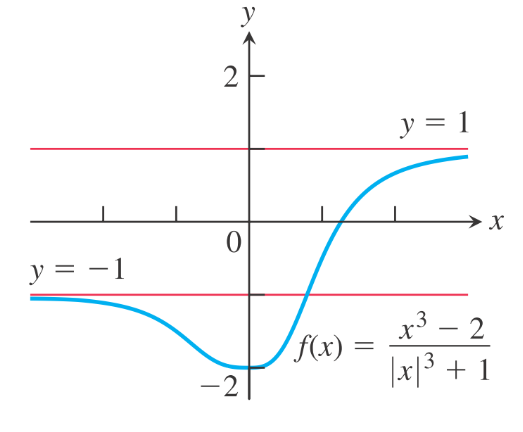
\includegraphics[width = 0.4\linewidth]{Images/infty limit.png}
     \caption{Graph of $\frac{x^3 + 2}{|x|^3 + 1}$}
\end{figure}

\subsection{Infinite Limits}
\begin{figure}[h!]
    \begin{subfigure}{.5\linewidth}
        \centering
        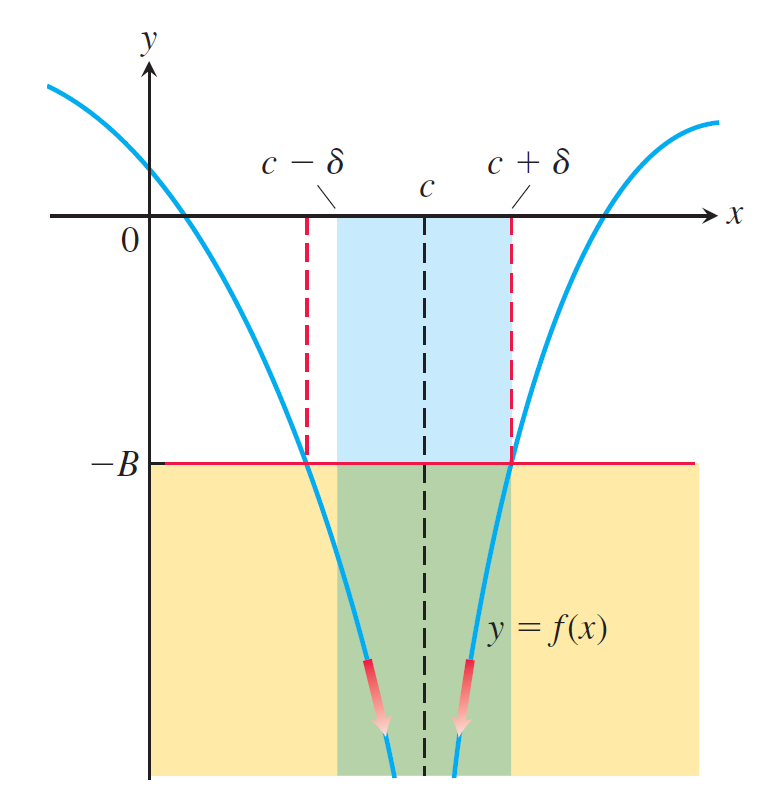
\includegraphics[width=0.9\linewidth]{Images/infty limit 2.png}
        \caption{Limit approaches negative infinity}
    \end{subfigure}
    \begin{subfigure}{0.5\linewidth}
        \centering
        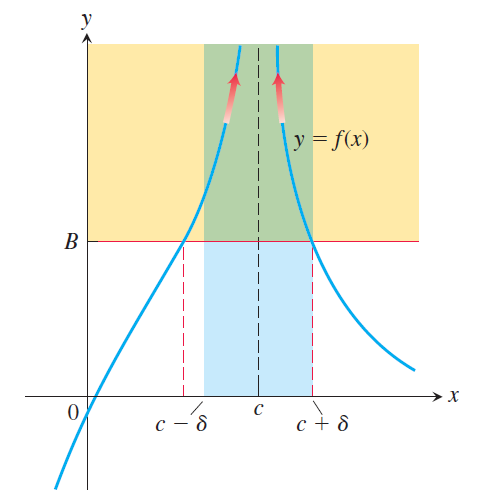
\includegraphics[width=0.9\linewidth]{Images/infty limit 3.png}
        \caption{Limit approaches positive infinity}
    \end{subfigure}
    \caption{Infinite Limits}
\end{figure} 
\paragraph{Definition} First, We say that $f(x)$ approaches infinity as $x$ approaches $c$, and write
\[
    \lim_{x \to c} f(x) = \infty
\]

if, for every number positive real number $B$ , there exists a corresponding number $\delta > 0$ such that for all $x$
\[
    0 < |x - c| < \delta \textrm{\tab} \Rightarrow \textrm{\tab} f(x) > B
\]
Second, We say that $f(x)$ approaches minus infinity as $x$ approaches $c$, and write
\[
    \lim_{x \to c} f(x) = - \infty
\]

if, for every number negative real number $-B$ , there exists a corresponding number $\delta > 0$ such that for all $x$
\[
    0 < |x - c| < \delta \textrm{\tab} \Rightarrow \textrm{\tab} f(x) < -B
\]

\paragraph{Note} Note that, when we say a limit = $\pm \infty$ limit laws still axis, that is the limit exists
if the left-side limit = right-side limit.

\paragraph{Example 1} Find
\[
    \lim_{x \to 2} \frac{x - 3}{x^2 - 4} 
\]

\begin{align*} 
    \lim_{x \to 2^{-}} \frac{x - 3}{x^2 - 4} = \frac{ - }{ - } = +\infty\, \\
    \lim_{x \to 2^{+}} \frac{x - 3}{x^2 - 4} = \frac{ - }{ + } = -\infty\, \\
\end{align*}

Since $\lim_{x \to 2^{-}} \frac{x - 3}{x^2 - 4} \neq \lim_{x \to 2^{+}} \frac{x - 3}{x^2 - 4}$, the limit does not exist.

\paragraph{Example 2} Find
\[
    \lim_{x \to -\infty} \frac{2x^5 - 6x^4 + 1}{3x^2 + x - 7} 
\]

\begin{align*} 
    \lim_{x \to -\infty} \frac{2x^5 - 6x^4 + 1}{3x^2 + x - 7} &=   \lim_{x \to -\infty} \frac{2x^5 - 6x^4 + 1}{3x^2 + x - 7} \cdot \frac{{\frac{1}{x^2}}}{\frac{1}{x^2}} \\
    &=  \lim_{x \to -\infty} \frac{2x^3 - 6x^2 + \frac{1}{x^2}}{3 + \frac{1}{x} - \frac{7}{x^2}} \\
    &= \frac{1}{3} \lim_{x \to -\infty} 2x^2(x - 3) \\
    &= -\infty
\end{align*}


\paragraph{Geometric Representation: Definition} While limit at infinity is related to horizontal asymtote, infinite limit
is related to vertical asymptote. \\ \\
\noindent
A line $x = a$ is a \textbf{vertical asymptote} of the graph of a function $y = f(x)$ if either
\[
    \lim_{x \to a^{+}} f(x) = \pm \infty \textrm{\tab} or \textrm{\tab} \lim_{x \to a^{-}} f(x) = \pm \infty 
\]

\subsection{Dominant Terms}
\paragraph{Definition} 
When considering functions made up of the sums, differences, products or quotients of different sorts of functions (polynomials, exponentials and logarithms), or 
different powers of the same sort of function we say that one function dominates the other and is called \textbf{dominant terms}. \\

\noindent
Dominant terms is useful for us to predict the function's behavior in certain condition of x. In polynomial functions, the dominant term is the function that has 
the highest degree. For example. $f(x) = 3x^4 + x^3 - 2x^2 + 7x - 5$ has $3x^4$ as the dominant term. In rational functions we can find the dominant term by modify the
form of the function as polynomial/quadratic/linear function plus the reminder. For example:
\[
    f(x) = \frac{x^2 + 3}{2x - 4} = \left(\frac{x}{2} + 1\right) + \left(\frac{1}{2x + 4}\right)
\]

For $|x|$ large, the dominant term is $x/2 + 1$ and for x close to 2, the dominant term is $1/2x + 4$
\subsection{Oblique Asymptote}
If the degree of the numerator of a rational function is 1 greater than the degree of the
denominator, the graph has an oblique or slant line asymptote. 

\paragraph{Definition}
The line given by $y = Ax + B$ is called an oblique asymptote of the graph of a function $y = f(x)$ if
\[
    \lim_{x \to \infty} (f(x) - Ax - B) = 0 \textrm{\tab or \tab} \lim_{x \to -\infty} (f(x) - Ax - B) = 0
\]

Suppose that $y = f(x)$ has an oblique asymptote $y = Ax + B$ as $x \to \infty$ then $f(x) - Ax - B \to 0$ as
$x \to \infty$. So 
\begin{align*} 
    \lim_{x \to \infty} \frac{f(x) - Ax - B}{x} = 0 \\
    \lim_{x \to \infty} \frac{f(x)}{x} - \lim_{x \to \infty} \frac{Ax}{x} +\lim_{x \to \infty} \frac{B}{x} = 0 \\
    A = \lim_{x \to \infty} \frac{f(x)}{x}
\end{align*}

Then, we have
\begin{align*} 
    \lim_{x \to \infty} (f(x) - Ax - B) = 0 \\
    \lim_{x \to \infty} f(x) - Ax - \lim_{x \to \infty} B = 0 \\
    B = \lim_{x \to \infty} f(x) - Ax \\
\end{align*}

Hence,
\[
    A = \lim_{x \to \infty} \frac{f(x)}{x} \textrm{\tab and \tab} B = \lim_{x \to \infty} f(x) - Ax
\]

\paragraph{Example} Find the oblique asymptote of
\[
    y = \frac{x^2 - 3}{2x - 4} 
\]

Let $y = Ax + B$ as the oblique asymptote of y, then we have
\begin{align*} 
    A &= \lim_{x \to \infty} \frac{f(x)}{x}\\
    &= \lim_{x \to \infty} \frac{x - \frac{3}{x}}{2x - 4} \frac{\frac{1}{x}}{\frac{1}{x}} \\
    &= \lim_{x \to \infty} \frac{1 - \frac{3}{x^2}}{2 - \frac{4}{x}} \\
    &= \frac{1}{2}
\end{align*}

Then we calculate B
\begin{align*} 
    B &= \lim_{x \to \infty} f(x) - Ax \\
    &= \lim_{x \to \infty} \frac{x^2 - 3}{2x - 4} \cdot \frac{x}{2} \\
    &= \lim_{x \to \infty} \frac{x^2 - 3 -\frac{x}{2}(2x - 4)}{2x - 4} 
    &= \lim_{x \to \infty} \frac{2x - 3}{2x - 4} \\
    &= 1 
\end{align*}

Hence, the oblique asymptote is $x/2 + 1$ \\ \\
We can also find the oblique asymptote by changing the form of the function to linear function plus the reminder using long division.

\begin{align*} 
    y &= \frac{x^2 - 3}{2x - 4} \\
    &= \left(\frac{x}{2} + 1\right) + \left(\frac{1}{2x + 4}\right)
\end{align*}

As $x \to \pm \infty$ the value of $f(x)$ will resemble the dominant term of the linear function $\left(\frac{x}{2} + 1\right)$

\section{Evaluating Limits}
\paragraph{Methods of Solving Limits} To solve limits, there are several methods we can use, such as:
\paragraph{Substitution} Substitute $c$ into $x$ directly. This applies if $f(x)$ is continuous at $c$. For example:
\[
    \lim_{x \to 2} x^2 = 2^2 = 4
\]

\paragraph{Factorization} This method is used to solve limit of rational functions, that is in the form of $p(x)/q(x)$ with
$p(x)$ and $q(x)$ are polynomials. First factorize the polynomials, then eliminate common factors from zero denominators. For example:
\[
    \lim_{x \to 2} \frac{x^2 - 4}{x - 2} =  \lim_{x \to 2} \frac{(x - 2)(x + 2)}{x - 2} = \lim_{x \to 2} x + 2 = 4
\]
\paragraph{Multiply with conjugate root} This method is used to solve limit of rational functions that have root function. 
Multiply the form with the conjugate of the root so that we can get a form where we can eliminate common factors from zero denominators.
For example:
\begin{align*} 
    \lim_{x \to 0} \frac{\sqrt{x^2 + 100} - 10}{x^2} &=  \lim_{x \to 0} \frac{(\sqrt{x^2 + 100} - 10)(\sqrt{x^2 + 100} + 10)}{x^2(\sqrt{x^2 + 100} + 10)} \\
    &= \lim_{x \to 0} \frac{x^2}{x^2(\sqrt{x^2 + 100} + 10)} \\
    &= \lim_{x \to 0} \frac{1}{\sqrt{x^2 + 100} + 10} \\
    &= \frac{1}{20}
\end{align*}

\paragraph{Using sandwich theorem} This method is used to solve limit with a special condition that satisfy the sandwich theorem
For example:
\begin{align*} 
    \lim_{x \to 0^{+}} x \floor*{\frac{1}{x}}
\end{align*}

\noindent
Let t = $1/x$ so that
\[
    \lim_{x \to 0^{+}} x \floor*{\frac{1}{x}} = \lim_{t \to \infty} \frac{1}{t} \floor*{t} 
\]

\noindent
Since, $\floor*{t}$ is a floor function that by definition:
\[
    t - 1 \leq \floor*{t} \leq t
\]
which gives,
\[
    1 - \frac{1}{t} \leq \frac{\floor*{t}}{t}  \leq 1
\]
\noindent
Since
\[
    \lim_{t \to \infty} 1 - \frac{1}{t} = 1 \textrm{ and } \lim_{t \to \infty} 1 = 1
\]
by sandwich theorem, $\lim_{x \to 0^{+}} x \floor*{\frac{1}{x}} = 1$
\paragraph{Substitute the variable} When we do substitution in a limit, we have to change all appearances of the original 
variable, which also includes the place under "lim". There we simply change the name of the variable, but the limit point 
itself must change according to the basic substitution equality. \\
For example:
\begin{align*} 
    \lim_{x \to \infty} x \sin{\frac{1}{x}}
\end{align*}

\noindent
Let $y = \frac{1}{x}$, so $y \to 0^{+}$ as $x \to \infty$
\begin{align*} 
    \lim_{x \to \infty} x \sin{\frac{1}{x}} & = \lim_{y \to 0^{+}} \frac{1}{y} \sin{y} \\
    & = \lim_{y \to 0^{+}} \frac{\sin{y}}{y} \\
    & = 1 \\
\end{align*}

\paragraph{Divide with highest degree denominator} This method can be used for limit as $x \to \pm \infty$. We can 
divide the numerator and denominator with the highest degree denominator and we can see the function's behavior as 
x approaches $\pm \infty$. For example,
\begin{align*} 
    \lim_{x \to \infty}\frac{3x^7 + 5x^2 - 1}{6x^3 - 7x + 3} &= \lim_{x \to \infty}\frac{3x^7 + 5x^2 - 1}{6x^3 - 7x + 3} \cdot \frac{\frac{1}{x^3}}{\frac{1}{x^3}} \\
    &= \lim_{x \to \infty}\frac{3x^4 + \frac{5}{x} - \frac{1}{x^3}}{6 - \frac{7}{x^2} + \frac{3}{x^3}} \\
    &= \infty
\end{align*}

\end{document}